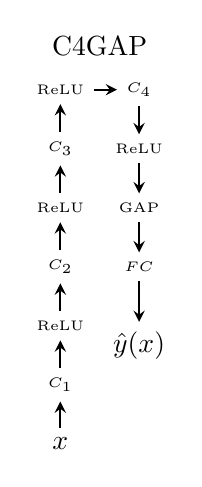
\begin{tikzpicture}

%%%%%%%%%%%%%%%%%%%%%%%%%%%%%%%%%%%%%%%%%%%%%%%%%%%%%%%%%%%%%%%%%
%%%%%%%%%%%%%%%%%%%%%%%%%%%%%%
\node []  (fntext)at (0.5,2.55) {C4GAP};

\node [] (output) at (1,-1.25){$\hat{y}(x)$};

\node [] (fc) at (1,-0.25){\tiny{$FC$}};
\draw [-stealth,thick]  (fc.south) -- (output.north);
\node [] (gap) at (1,0.5){\tiny{GAP}};
\draw [-stealth,thick]  (gap.south) -- (fc.north);


\node [] (relu4) at (1,1.25){\tiny{ReLU}};
\draw [-stealth,thick]  (relu4.south) -- (gap.north);
\node [] (c4) at (1,2.0){\tiny{$C_4$}};
\draw [-stealth,thick]  (c4.south) -- (relu4.north);


\node [] (relu3) at (0,2.0){\tiny{ReLU}};
\draw [-stealth,thick]  (relu3.east) -- (c4.west);
\node [] (c3) at (0,1.25){\tiny{$C_3$}};
\draw [-stealth,thick]  (c3.north) -- (relu3.south);



\node [] (relu2) at (0,0.5){\tiny{ReLU}};
\draw [-stealth,thick]  (relu2.north) -- (c3.south);
\node [] (c2) at (0,-0.25){\tiny{$C_2$}};
\draw [-stealth,thick]  (c2.north) -- (relu2.south);


\node [] (relu1) at (0,-1.0){\tiny{ReLU}};
\draw [-stealth,thick]  (relu1.north) -- (c2.south);
\node [] (c1) at (0,-1.75){\tiny{$C_1$}};
\draw [-stealth,thick]  (c1.north) -- (relu1.south);

\node [] (x) at (0,-2.5){$x$};
\draw [-stealth,thick ]  (x.north) -- (c1.south);


%%%%%%%%%%%%%%%%%%%%%%%%%%%%%%%%%%%%%%%%%%%%%%%%%%%%%%%%%%%%%%%%%


	
\end{tikzpicture}

